%%%%%%%%%%%%%%%%%%%%%%%%%%%%%%%%%%%%%%%%%%%%%%%%%%%%%%%%%%%%%%%%%%%%%%
%% Copyright (c) 2016 Carsten Wulff Software, Norway
%% %%%%%%%%%%%%%%%%%%%%%%%%%%%%%%%%%%%%%%%%%%%%%%%%%%%%%%%%%%%%%%%%%%%
%% Created       : wulff at 2016-11-5
%% %%%%%%%%%%%%%%%%%%%%%%%%%%%%%%%%%%%%%%%%%%%%%%%%%%%%%%%%%%%%%%%%%%%
%% This program is free software: you can redistribute it and/or modify
%% it under the terms of the GNU General Public License as published by
%% the Free Software Foundation, either version 3 of the License, or
%% (at your option) any later version.
%%
%% This program is distributed in the hope that it will be useful,
%% but WITHOUT ANY WARRANTY; without even the implied warranty of
%% MERCHANTABILITY or FITNESS FOR A PARTICULAR PURPOSE.  See the
%% GNU General Public License for more details.
%%
%% You should have received a copy of the GNU General Public License
%% along with this program.  If not, see <http://www.gnu.org/licenses/>.
%%%%%%%%%%%%%%%%%%%%%%%%%%%%%%%%%%%%%%%%%%%%%%%%%%%%%%%%%%%%%%%%%%%%%%
%\documentclass[final,11pt]{IEEEtran}
\documentclass[crop,border=0pt]{standalone}
\usepackage{times}


%\usepackage{placeins}
\usepackage{upgreek}
\usepackage{amssymb,amsmath}
\usepackage{cite}
\usepackage{verbatim}
\usepackage{listings}
\usepackage{xcolor}
\usepackage{flafter}
\usepackage{booktabs}
\usepackage{url}
\usepackage{ textcomp }

\hyphenation{op-tical net-works semi-conduc-tor}


% -JSON styel

%\definecolor{darkGreen}{rgb}{0,0.2097,0}
%\newcommand{\myfigwidth}{\linewidth}
%\newcommand{\myfigwidtha}{\linewidth}
%\newcommand{\myfigwidthl}{\textwidth}
%\newcommand{\myfigwidthc}{0.6\linewidth}


\newcommand{\myfigwidtha}{3.3in}
\newcommand{\myfigwidthl}{7in}
\newcommand{\myfigwidthc}{2in}
%\newcommand{\myfigwidthe}{3.2in}
%\newcommand{\myfigwidthb}{5in}

\newcommand{\myfigname}{fig_}
\newcommand{\reg}[2]{{\figurename} \ref{#1}(#2)}
\newcommand{\req}[1]{{\figurename} \ref{#1}}
%\newcommand{\myeqname}{eq:}
%\newcommand{\req}[1]{(\ref{\myeqname#1})}

\definecolor{armygreen}{rgb}{0, 0.5, 0}
\newcommand{\missing}[1]{{ #1}}
\newcommand{\edit}[1]{{ #1}}
\newcommand{\secedit}[1]{{ #1}}
\newcommand{\deleted}[1]{{ #1}}
\newcommand{\moved}[1]{{ #1}}

%\newcommand{\missing}[1]{{\color{red} #1}}
%\newcommand{\edit}[1]{{\color{red} #1}}
%\newcommand{\secedit}[1]{{\color{armygreen} #1}}
%\newcommand{\deleted}[1]{{\color{violet} #1}}
%\newcommand{\moved}[1]{{\color{blue} #1}}

\newcommand{\SD}{Sigma-Delta }
\newcommand{\eqn}[1]{
  \begin{math}
    #1
  \end{math}}

\newcommand\JSONnumbervaluestyle{\color{blue}}
\newcommand\JSONstringvaluestyle{\color{red}}



\newif\ifcolonfoundonthisline

\makeatletter

\lstdefinestyle{json}
{
  showstringspaces    = false,
  keywords            = {false,true},
  alsoletter          = 0123456789.,
  morestring          = [s]{"}{"},
  stringstyle         = \ifcolonfoundonthisline\JSONstringvaluestyle\fi,
  MoreSelectCharTable =%
  \lst@DefSaveDef{`:}\colon@json{\processColon@json},
  basicstyle          = \fontsize{7}{7}\ttfamily,
  keywordstyle        = \fontsize{7}{7}\ttfamily\bfseries,
}

% flip the switch if a colon is found in Pmode
\newcommand\processColon@json{%
  \colon@json%
  \ifnum\lst@mode=\lst@Pmode%
  \global\colonfoundonthislinetrue%
  \fi
}

\lst@AddToHook{Output}{%
  \ifcolonfoundonthisline%
  \ifnum\lst@mode=\lst@Pmode%
  \def\lst@thestyle{\JSONnumbervaluestyle}%
  \fi
  \fi
  % override by keyword style if a keyword is detected!
  \lsthk@DetectKeywords%
}

% reset the switch at the end of line
\lst@AddToHook{EOL}%
{\global\colonfoundonthislinefalse}

\makeatother

% \lstset{  basicstyle=\tiny}

% \lstset{
% basicstyle=\fontsize{11}{13}\selectfont\ttfamily
% }


\lstset{language=Java}




%\usepackage[paperwidth=\maxdimen,paperheight=\maxdimen]{geometry}


\usepackage{tikz,pgfplots}
\usepackage{ifthen}
\usepackage{calc}
\usetikzlibrary{patterns}
%\usepackage[tightpage,active]{preview}
\usetikzlibrary{circuits.logic.US}
\usetikzlibrary{circuits.ee.IEC}
\usepgflibrary{shapes.arrows}
\usepgflibrary{arrows}
\usepackage{circuitikz}


% circuitikz draws bipole outlines (resistors, diodes, capacitors) at
% bipoles/thickness times the ambient line width, and the default is 2.
% That makes a circuitikz resistor visibly heavier than the wire it sits
% on, and heavier than the hand rolled zig-zag in ckt_lib.tex. One is the
% house width: everything is drawn at the environment's own thickness.
% Arrow tips: one filled tip everywhere, set through the '>' knob so a
% figure only ever writes ->, <- or <->. Latex (from arrows.meta)
% scales with the line width, so it stays in proportion if a drawing
% is ever set thicker or thinner than the house 'thick'.
\usetikzlibrary{arrows.meta}
\tikzset{>={Latex}}

\ctikzset{bipoles/thickness=1}
\ctikzset{tripoles/mos style/arrows}
\ctikzset{tripoles/pmos style/emptycircle}
%\PreviewEnvironment{circuitikz}
\pagestyle{empty}


\tikzstyle{cicfill}=[minimum size=1.4em]
\tikzstyle{stuff_fill}=[rectangle,fill=white,minimum size=1.4em]

\newcommand{\grayOne}{0.3 }
\newcommand{\grayTwo}{0.15 }
\newcommand{\grayThree}{0.26 }
\newcommand{\grayFour}{0.41 }
\newcommand{\grayFive}{0.61 }
\newcommand{\graySix}{0.85 }

%- Gray tone
%\definecolor{active}{rgb}{\graySix,\graySix,\graySix}
%\definecolor{poly}{rgb}{\grayFive,\grayFive,\grayFive}
%\definecolor{contact}{rgb}{\graySix,\graySix,\graySix}
%\definecolor{mOne}{rgb}{\grayFour,\grayFour,\grayFour}
%\definecolor{mTwo}{rgb}{\graySix,\graySix,\graySix}
%\definecolor{mThree}{rgb}{\grayThree,\grayThree,\grayThree}
%\definecolor{mFour}{rgb}{\grayTwo,\grayTwo,\grayTwo}

\definecolor{grey}{rgb}{1,1,1}
\definecolor{lightgrey}{rgb}{\grayFour,\grayFour,\grayFour}
\definecolor{active}{rgb}{0.4,1,0.6}
\definecolor{poly}{rgb}{1.0,0.5,0.5}
\definecolor{cut}{rgb}{0.91,0.91,0}
\definecolor{mOne}{rgb}{0.36,0.36,1}
\definecolor{mTwo}{rgb}{0.655,0.655,0}
\definecolor{mThree}{rgb}{0.3,1,1}
\definecolor{mFour}{rgb}{0,0.2097,0}
\begin{document}


% Power system of the nRF54L15, after the regulator configuration in the
% product specification. VDD (1.7 V - 3.6 V, decoupled by CVDD) feeds
% VREGMAIN directly, and a second VDD rail feeds the GPIO blocks and the
% RRAM. VREGMAIN holds a DC/DC and an LDO. The DC/DC switches the DCC
% pin through the external inductor LDCC onto DECD, the low voltage
% digital supply (decoupled by CDECD) that powers every power domain:
% MCU, CRACEN, RRAM, peripherals, low power and radio. The LDO drives
% DECA, the analog supply for the radio, which is also fed from DECD
% through the ferrite bead FB. DECRF, the PA and LNA supply, is tied to
% DECA outside the chip. Drawn as a ferrite bead with the inductor
% symbol. Redrawn so the book does not carry the datasheet figure.

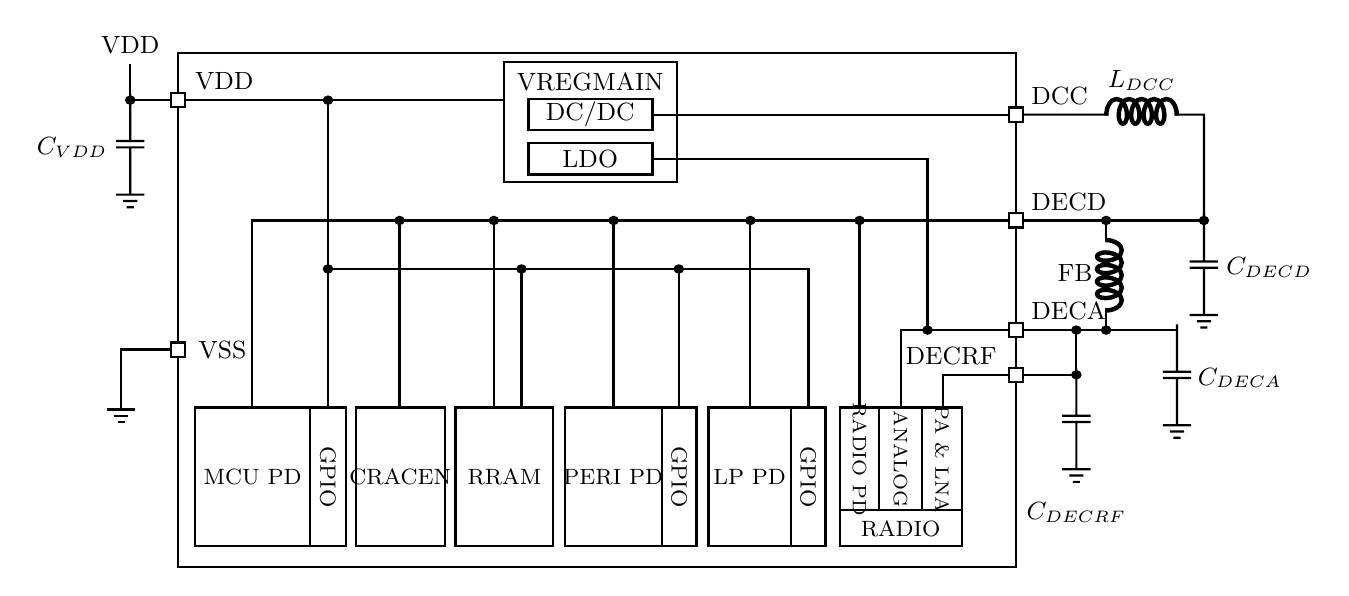
\begin{tikzpicture}[thick, x=0.9cm, y=0.8cm, font=\small]

  

\newcommand{\grid}{1.6}


% ---------------------------------------------------------
% Elementals
% ---------------------------------------------------------

\newcommand{\cicVcIsDown}[1]{
  ++(0,\grid) to []
}

\newcommand{\hresistor}[1]{
  ++(0,0) coordinate (cStart)
  to [short,-] ++(0.5,0)
  to [short,-] ++(0.05,0.1)
  to [short,-] ++(0.1,-0.2)
  to [short,-] ++(0.1,0.2)
  to [short,-] ++(0.1,-0.2)
  to [short,-] ++(0.1,0.2)
  to [short,-] ++(0.1,-0.2)
  to [short,-] ++(0.05,0.1)
  to [short,-] ++(0.5,0)
  coordinate (resEnd)
  ++(-0.8,0.1)
  node [anchor=south] {#1}
  (resEnd)
}

\newcommand{\vresistor}[1]{
  ++(0,0) coordinate (cStart)
  to [short,-] ++(0,0.5)
  to [short,-] ++(0.1,0.05)
  to [short,-] ++(-0.2,0.1)
  to [short,-] ++(0.2,0.1)
  to [short,-] ++(-0.2,0.1)
  to [short,-] ++(0.2,0.1)
  to [short,-] ++(-0.2,0.1)
  to [short,-] ++(0.1,0.05)
  to [short,-] ++(0,0.5)
  coordinate (resEnd)
  ++(0.1,-0.8)
  node [anchor=west] {#1}
  (resEnd)
}

\newcommand{\vimpedance}[1]{
  ++(0,0) coordinate (cStart)
  -- ++(0,0.5)
  -- ++(0.25,0)
  -- ++(0,0.6)
  -- ++(-0.50,0)
  -- ++(-0,-0.6)
  -- ++(0.25,0)
  ++(0,0.6)
  -- ++(0,0.5)
  coordinate (impEnd)
  ++(0,-0.8)
  node [anchor=center] {#1}
  (impEnd)
}

\newcommand{\himpedance}[1]{
  ++(0,0) coordinate (cStart)
  -- ++(0.5,0)
  -- ++(0,0.25)
  -- ++(0.6,0)
  -- ++(-0.0,-0.5)
  -- ++(-0.6,-0)
  -- ++(0.0,0.25)
  ++(0.6,0)
  -- ++(0.5,0)
  coordinate (impEnd)
  ++(-0.8,-0)
  node [anchor=center] {#1}
  (impEnd)
}

\newcommand{\vnmos}[1]{
 to [Tnmos, n=#1, l=#1] ++(0,\grid)
}

\newcommand{\vmnmos}[1]{
 to [Tnmos, n=#1, l=#1,mirror] ++(0,\grid)
}

\newcommand{\vpmos}[1]{
 to [Tpmos, n=#1, l=#1] ++(0,\grid)
}

\newcommand{\vvsource}[1]{
  to [V,l_=#1] ++(0,-\grid*1.5)
}

\newcommand{\vmpmos}[1]{
 to [Tpmos, n=#1, l=#1,mirror] ++(0,\grid)
}

\newcommand{\lvnmos}[2]{
 to [Tnmos, n=#1] ++(0,\grid) coordinate (cicmos) \if \relax\detokenize{#2}\relax \else (#1.gate)
 \portIn{#2} \fi (cicmos)
}

\newcommand{\lvmnmos}[2]{
  to [Tnmos, n=#1,mirror] ++(0,\grid) coordinate (cicmos) \if \relax\detokenize{#2}\relax \else (#1.gate)
 \portmIn{#2} \fi (cicmos)
}

\newcommand{\hinv}[1]{
  ++(0.7,0) node[not port] (#1) {} ++(0.7,0)

}

\newcommand{\lvpmos}[2]{
  to [Tpmos, n=#1] ++(0,\grid) coordinate (cicmos) (#1.gate)  \if \relax\detokenize{#2}\relax \else (#1.gate)
 \portIn{#2} \fi (cicmos)
}

\newcommand{\lvmpmos}[2]{
  to [Tpmos, n=#1,mirror] ++(0,\grid) coordinate (cicmos)  \if \relax\detokenize{#2}\relax \else (#1.gate)
 \portmIn{#2} \fi (cicmos)
}


\newcommand{\vsupply}{
  ++(0,0) coordinate (vSupplyStart)
  -- ++(0,\grid/4)
  ++(-\grid/8,-\grid/16) to [short,-] ++(\grid/4,\grid/8)
  (vSupplyStart)
}

\newcommand{\vground}{
  ++(0,0) coordinate (cStart)
  ++(-0.2,0) to [short,-] ++(0.4,0)
  ++(-0.3,-0.1) to [short,-] ++(0.2,0)
  ++(-0.15,-0.1) to [short,-] ++(0.1,0)
  %++(-0.5,0.05) to [short,-] ++(0.5,0)
  (cStart)
}


\newcommand{\vcapacitor}[1]{
  ++(0,0) coordinate (cStart)
  to [short,-] ++(0,0.75)
  ++(-0.2,0) to [short,-] ++(0.4,0)
  ++(-0.4,0.1) to [short,-] ++(0.4,0)
  ++(-0.2,0)
  to [short,-] ++(0,0.75)
  coordinate (capEnd)
  ++(0.1,-0.8)
  node [anchor=west] {#1}
  (capEnd)
}

\newcommand{\hcapacitor}[1]{
  ++(0,0) coordinate (cStart)
  to [short,-] ++(0.75,0)
  ++(0,-0.2) to [short,-] ++(0,0.4)
  ++(0.1,-0.4) to [short,-] ++(0,0.4)
  ++(0,-0.2)
  to [short,-] ++(0.75,0)
  coordinate (capEnd)
  ++(-0.8,0.1)
  node [anchor=south] {#1}
  (capEnd)
}


\newcommand{\portDiffIn}[1]{
 ++(0,0) coordinate (cStart)
 to [short,o-] ++(0,0)
 node [anchor=north] {$+$}
 ++(0,-1.6)
  to [short,o-] ++(0,0)
  node [anchor=south] {$-$}
  ++(0,0.8)
  node [anchor=center] {#1} ++(0,0)
  (cStart)
}

\newcommand{\portDiffComplexIn}[1]{
 ++(0,0) coordinate (cicComplexStart)
 \portDiffIn{I #1}
 (cicComplexStart)
 ++(0,-\grid*3)
 \portDiffIn{Q #1}
 (cicComplexStart)
}

\newcommand{\portDiffComplexOut}[1]{
  ++(0,0) coordinate (cicComplexStart)
 \portDiffOut{I #1}
 (cicComplexStart)
 ++(0,-\grid*3)
 \portDiffOut{Q #1}
 (cicComplexStart)
}


\newcommand{\portDiffOut}[1]{
 ++(0,0) coordinate (cStart)

 to [short,-o] ++(0.5,0)
 node [anchor=north] {$+$}
 ++(-0.5,-1.6)
 to [short,-o] ++(0.5,0)
 node [anchor=south] {$-$}
 ++(0,0.8)
 node [anchor=center] {#1} ++(0,0)
 (cStart)
}

\newcommand{\portIn}[1]{
 ++(0,0) coordinate (cStart)
  node [anchor=east] {#1} ++(0,0)
  to [short,o-] ++(0,0)
}

\newcommand{\portmIn}[1]{
 ++(0,0)
  node [anchor=west] {#1} ++(0,0)
  to [short,o-] ++(0,0)
}

\newcommand{\portBox}{
  ++(-0.1,0.2) -- ++(0.2,0)
  -- ++(0,-0.2)
  -- ++(-0.2,0)
  -- ++(0,0.2)
  -- ++(0.2,-0.2)
  ++(-0.2,0) -- ++(0.2,0.2)
  ++(-0.1,0)
}

\newcommand{\portOut}[1]{
  ++(0,0) coordinate (cStart)
  to [short,*-o] ++(0.5,0)
  node [anchor=west] {#1}
}

\newcommand{\portOutDown}[1]{
  ++(0,0) coordinate (cStart)
  to [short,-o] ++(0,-\grid/2)
  node [anchor=west] {#1}
}

\newcommand{\curDown}[1]{
  ++(0,0) [short,i>=#1] ++(0,-\grid/2)
}

\newcommand{\portCurDown}[1]{
  ++(0,0) [short,i>=#1] ++(0,-\grid/2)
  node [anchor=west] {#1}
}

\newcommand{\cicAdd}{
  ++(0,0) ++(\grid/8,0) node [anchor=center] {+} circle (\grid/8) ++(\grid/8,0)
}

\newcommand{\cicH}[1]{
  ++(0,0) ++(\grid/4,0) node [anchor=center] {#1} ++(-\grid/4,-\grid/4)
  rectangle ++(\grid/2,\grid/2) ++(0,-\grid/4)
}


%---------------------------------------------------------
% Digital gates
% ---------------------------------------------------------
% Hand-rolled to match the hand-drawn originals: straight NAND
% shoulders with a round cap, a swept full-bodied NOR, and generous
% bubbles. The stock circuitikz ports are squat by comparison and are
% not used. Path fragments: entry at the gate's centre-left on the
% output axis; exit past the output. Exported coordinates:
% (#1_in1) (#1_in2) (#1_out).

\newcommand{\cicNand}[1]{
  ++(0,0.32) coordinate (#1_in1)
  ++(0,-0.64) coordinate (#1_in2)
  ++(0,-0.28)
  -- ++(0,1.2) -- ++(0.5,0)
  .. controls +(0.45,-0.02) and +(0,0.3) .. ++(0.68,-0.6)
  .. controls +(0,-0.3) and +(0.45,0.02) .. ++(-0.68,-0.6)
  -- ++(-0.5,0)
  ++(1.28,0.6) circle (0.1)
  ++(0.1,0) coordinate (#1_out)
}

\newcommand{\cicAnd}[1]{
  ++(0,0.32) coordinate (#1_in1)
  ++(0,-0.64) coordinate (#1_in2)
  ++(0,-0.28)
  -- ++(0,1.2) -- ++(0.5,0)
  .. controls +(0.45,-0.02) and +(0,0.3) .. ++(0.68,-0.6)
  .. controls +(0,-0.3) and +(0.45,0.02) .. ++(-0.68,-0.6)
  -- ++(-0.5,0)
  ++(1.18,0.6) coordinate (#1_out)
}

\newcommand{\cicNor}[1]{
  ++(0,0.32) coordinate (#1_in1) to [short,-] ++(0.2,0) ++(-0.2,0)
  ++(0,-0.64) coordinate (#1_in2) to [short,-] ++(0.2,0) ++(-0.2,0)
  ++(0,-0.28)
  .. controls +(0.22,0.35) and +(0.22,-0.35) .. ++(0,1.2)
  .. controls +(0.65,0.02) and +(-0.35,0.4) .. ++(1.5,-0.6)
  .. controls +(-0.35,-0.4) and +(0.65,-0.02) .. ++(-1.5,-0.6)
  ++(1.6,0.6) circle (0.1)
  ++(0.1,0) coordinate (#1_out)
}

\newcommand{\cicOr}[1]{
  ++(0,0.32) coordinate (#1_in1) to [short,-] ++(0.2,0) ++(-0.2,0)
  ++(0,-0.64) coordinate (#1_in2) to [short,-] ++(0.2,0) ++(-0.2,0)
  ++(0,-0.28)
  .. controls +(0.22,0.35) and +(0.22,-0.35) .. ++(0,1.2)
  .. controls +(0.65,0.02) and +(-0.35,0.4) .. ++(1.5,-0.6)
  .. controls +(-0.35,-0.4) and +(0.65,-0.02) .. ++(-1.5,-0.6)
  ++(1.5,0.6) coordinate (#1_out)
}

\newcommand{\cicInv}[1]{
  ++(0,0) coordinate (#1_in)
  ++(0,-0.55) -- ++(0,1.1) -- ++(0.9,-0.55) -- ++(-0.9,-0.55)
  ++(1.0,0.55) circle (0.1)
  ++(0.1,0) coordinate (#1_out)
}

\newcommand{\cicBuf}[1]{
  ++(0,0) coordinate (#1_in)
  ++(0,-0.55) -- ++(0,1.1) -- ++(0.9,-0.55) -- ++(-0.9,-0.55)
  ++(0.9,0.55) coordinate (#1_out)
}

%---------------------------------------------------------
% OTA
% ---------------------------------------------------------

% Current mirror OTA

\newcommand{\cicOtaCM}{
  ++(0,0) coordinate (cicOtaStart)

  \vground
  \vnmos{M0}
  %Left branch
  coordinate (cicOtaSource)
  to [short,-] ++(-\grid/2,0)
  \vnmos{M1}
  to [short,-] ++(0,\grid/4)
  coordinate (cicOta_vbpp)
  \vpmos{M3}
  coordinate (cicOtaSupplyLeft)
  to [short,-] ++(\grid/2,0)
  \vsupply
  to [short,-] ++(\grid/2,0)
  coordinate (cicOtaSupplyRight)

  % Right branch
  (cicOtaSource)
  to [short,-] ++(\grid/2,0)
  \vmnmos{M2}
  to [short,-] ++(0,\grid/4)
  coordinate (cicOta_vbpn)
  \vmpmos{M4}
  to [short,-] ++(-\grid/2,0)

  % Current mirror left
  (cicOtaStart)
  ++(-\grid*2,-\grid)
  \vground
  \vmnmos{M5}
  to [short,-] ++(0,\grid*1.5)
  coordinate (cicOta_outp)
  to [short,-] ++(0,\grid*0.75)
  \vmpmos{M6}
  -- (cicOtaSupplyLeft)

  % Current mirror left
  (cicOtaStart)
  ++(\grid*2,-\grid)
  \vground
  \vnmos{M7}
  to [short,-] ++(0,\grid*1.5)
  coordinate (cicOta_outn)
  to [short,-] ++(0,\grid*0.75)
  \vpmos{M8}
  -- (cicOtaSupplyRight)



  (M5.gate) -- (M7.gate) ++(-\grid*1.4,0) to [short,o-] ++(0,0) node
  [anchor=south] {$V_{cmb}$}
  (M6.gate) -- (M3.gate)
  (M4.gate) -- (M8.gate)
  (M3.gate) |- (cicOta_vbpp)
  (M4.gate) |- (cicOta_vbpn)
  
  (M0.gate) to [short,o-] ++(0,0) node [anchor=east] {$V_{bn}$}
  (M1.gate) to [short,o-] ++(0,0) node [anchor=east] {$V_{ip}$}
  (M2.gate) to [short,-o] ++(0,0) node [anchor=west] {$V_{in}$}

  (cicOta_outn) to [short,-o] ++(\grid/4,0) node [anchor=west] {$V_{outn}$}
  (cicOta_outp) to [short,-o] ++(-\grid/4,0) node [anchor=east] {$V_{outp}$}
  %\vmpmos{m4}

}

\newcommand*{\cicOta}{

  ++(0,0) coordinate (cicOta_inp)

  % Positive input
  to [short,-] ++(0.5,0)
  node [anchor=west] {$+$}

  % Negative input
  to [short,-] ++(0,-\grid)
  node [anchor=west] {$-$}

  to [short,-] ++(-0.5,0)
  coordinate (cicOta_inn)
  ++(0.5,0)

  % Bottom
  to [short,-] ++(0,-0.4)
  to [short,-] ++(1.2,0)
  to [short,-] ++(0.4,0.3)
  -- ++(0,0.1)

  % Right
  node [anchor=east] {$+$}
  -- ++(0.5,0)
  coordinate (cicOta_outp)
  ++(-0.5,0)
  to [short,-] ++(0,1.6)
  node [anchor=east] {$-$}
  -- ++(0.5,0)

  coordinate (cicOta_outn)
  ++(-0.5,0)

  % Top
  -- ++(0,0.1)
  -- ++(-0.4,0.3)
  -- ++(-1.2,0)
  -- ++(0,-0.4)
  (cicOta_inp)
}

\newcommand*{\cicOtaSSWP}[2]{

  ++(0,0) coordinate (cicOtaS_inp)

  % Positive input
  to [short,-] ++(0.5,0)
  node [anchor=west] {#1}

  % Negative input
  to [short,-] ++(0,-\grid/2)
  node [anchor=west] {#2}

  to [short,-] ++(-0.5,0)
  coordinate (cicOtaS_inn)
  ++(0.5,0)

  % Bottom
  to [short,-] ++(0,-0.4)
  to [short,-] ++(\grid,\grid/2)

  % Right
  -- ++(0.5,0)
  coordinate (cicOtaS_out)
  ++(-0.5,0)

  to [short,-] ++(-\grid,\grid/2)

  -- ++(0,-0.5)
  % Top
  (cicOtaS_inp)
}


\newcommand*{\cicOtaSWP}[4]{

  ++(0,0) coordinate (cicOta_inp)

  % Positive input
  to [short,-] ++(0.5,0)
  node [anchor=west] {#1}

  % Negative input
  to [short,-] ++(0,-\grid)
  node [anchor=west] {#2}

  to [short,-] ++(-0.5,0)
  coordinate (cicOta_inn)
  ++(0.5,0)

  % Bottom
  to [short,-] ++(0,-0.4)
  to [short,-] ++(1.2,0)
  to [short,-] ++(0.4,0.3)
  -- ++(0,0.1)

  % Right
  node [anchor=east] {#3}
  -- ++(0.5,0)
  coordinate (cicOta_outp)
  ++(-0.5,0)
  to [short,-] ++(0,1.6)
  node [anchor=east] {#4}
  -- ++(0.5,0)

  coordinate (cicOta_outn)
  ++(-0.5,0)

  % Top
  -- ++(0,0.1)
  -- ++(-0.4,0.3)
  -- ++(-1.2,0)
  -- ++(0,-0.4)
  (cicOta_inp)
}


%---------------------------------------------------------
% Filters
% ---------------------------------------------------------

\newcommand{\filtLP}[2]{
  \hresistor{#1}
  ++(0,-1.6)
  \vground
  \vcapacitor{#2}
}


\newcommand{\filtHP}[2]{
  \hcapacitor{#1}
  ++(0,-1.6)
  \vground
  \vresistor{#2}
}


\newcommand{\filtActLP}[2]{

  +(0,0) coordinate (cicStart)
  \hresistor{#1}
  \cicOta
  (cicOta_inp) to [short,*-] ++(0,1)
  -- ++(0.5,0)
  \hcapacitor{#2}
  -| (cicOta_outn)
  (cicOta_inn) -- ++(0,-0.1)\vground
  (cicOta_outn)
}

\newcommand{\filtActZ}[2]{
  ++(0,0) coordinate (cicStart)
  \himpedance{#1}
  \cicOta
  (cicOta_inp) to [short,*-] ++(0,\grid/2)
  -- ++(0.5,0)
  \himpedance{#2}
  -| (cicOta_outn)
  (cicOta_inn) -- ++(0,-0.1)\vground
  (cicOta_outn)
}


\newcommand{\filtActDiffZ}[2]{
  ++(0,0) coordinate (cicStart)
  \himpedance{#1}
  \cicOta
  (cicOta_inp)
  to [short,*-] ++(0,\grid/2)
  -- ++(0.5,0)
  \himpedance{#2}
  -| (cicOta_outn)
  to [short,*-] ++(0,0)
  (cicOta_inn) ++(-1.6,0)
  \himpedance{#1}
  to [short,*-] ++(0,-\grid/2)
  -- ++(0.5,0)
  \himpedance{#2}
  -| (cicOta_outp)
  to [short,*-] ++(0,0)
  (cicOta_outn)
}

\newcommand{\filtActComplexDiffZOne}[1]{
  ++(0,0) coordinate (cicStart)
  \filtActDiffZ{#1}{#1}
  (cicOta_inp)
  ++(-\grid,0)
  coordinate (cicComplex_in2)
  ++(0,+\grid/2)
  coordinate (cicComplex_in1)
  \himpedance{#1}
  (cicOta_inn)
  ++(-\grid,0)
  coordinate (cicComplex_in3)
  ++(0,-\grid/2)
  coordinate (cicComplex_in4)
  \himpedance{#1}
  (cicOta_inp)
}

\newcommand{\filtActComplexDiffZ}[1]{
   ++(0,0) coordinate (cicStart)
    ++(\grid/2,0)
    \filtActComplexDiffZOne{Z}
    (cicComplex_in1) coordinate (cicI_in1)
    (cicComplex_in2) coordinate (cicI_in2)
    (cicComplex_in3) coordinate (cicI_in3)
    (cicComplex_in4) coordinate (cicI_in4)
    (cicOta_outn) coordinate(cicI_outn)
    (cicI_in2)
    ++(0,-\grid*3)
    \filtActComplexDiffZOne{Z}
    (cicComplex_in1) coordinate (cicQ_in1)
    (cicComplex_in2) coordinate (cicQ_in2)
    (cicComplex_in3) coordinate (cicQ_in3)
    (cicComplex_in4) coordinate (cicQ_in4)

    (cicI_in2) -- ++(-\grid/2,0) ++(\grid/4,0)
    to [short,*-] (cicQ_in1)

    (cicI_in3) -- ++(-\grid/2,0) ++(\grid/4,0)
    to [short,*-] (cicQ_in4)

    (cicQ_in2) -- ++(-\grid/2,0) ++(\grid/4,0)
    to [short,*-] (cicI_in1)

    (cicQ_in3) -- ++(-\grid/2,0) ++(\grid/4,0)
    to [short,*-] (cicI_in4)

    (cicI_outn)

}



%---------------------------------------------------------
% Transistors
%---------------------------------------------------------

\newcommand{\trNmos}{

++(0,0) coordinate (cStart)
to [Tnmos, n=mn1, l=$M_{1}$] ++(0,1.6)
(mn1.gate) to [short,o-] ++(0,0) node [anchor=east] {$Gate$}
(mn1.drain) to [short,o-] ++(0,0) node [anchor=east] {$Drain$}
(mn1.source) to [short,o-] ++(0,0) node [anchor=east] {$Source$}
;
}


\newcommand{\trSmallSignal}{ % Incomplete
    ++(0,0) coordinate (cStart) to [short,o-] ++(1,0) node [anchor=north] {$+$} ++(0,-0.8)
    node [anchor=east] {$v_i$}
     (cStart)    ++(0,-1.6) node [rground] {} to [short] ++(1,0) node [anchor=south] {$-$}
    (cStart) ++(2,0)
    to [cI, n=mn1, l=$gm_{1} \times v_i$] ++(0,-1.6)
    to [short] ++(3,0) \vresistor{$r_o$}
    node [anchor=south] {$v_o$}
    to [short] ++(-3.0,0)

}


%---------------------------------------------------------
% ESD
%---------------------------------------------------------

\newcommand{\esdGgnmos}{

++(0,0) coordinate (esdStart)
node [ground,rotate=-90,anchor=west] {}     to [Tnmos,
  n=mn1, l=$M_{1}$] ++(0,3.2) to [short,-*] ++(0,0)
coordinate (top) to
[short,-o] ++(0.5,0)  node [anchor=west] {To pin}

(top) to [short,-o] ++(-1,0) node [anchor=east] {To core}
(mn1.gate) to [short,-] ++(-1,0) ++(0,-1.6) coordinate (esdRbot)
\vresistor{} (esdRbot) node [ground,rotate=-90,anchor=west] {}
(esdStart)

}



%---------------------------------------------------------
%  Analog Question
% ---------------------------------------------------------

\newcommand{\anaQuestion}{
          +(0,0) coordinate (cStart)
          node [ground,rotate=-90,anchor=west] {}     to [Tnmos,
            n=mn1, l=$M_{1}$,mirror] ++(0,1.6) to [short]
          ++(0,3.2) node [rground,yscale=-1] {} to [I,l=$20 \mu A$,] ++(0,-1.6)

          (cStart) ++(4,0)
          node [ground,rotate=-90,anchor=west] {}     to [Tnmos,
            n=mn2, l=$M_{2}$] ++(0,1.6) to [short,-o] ++(0,0.8)
          node [short,anchor=west] {$V_X$} to [short] ++(0,0.8)
          to [Tnmos, n=mn3, l=$M_{3}$] ++(0,1.6)
          node [rground,yscale=-1] {} ++(0,0.4) node [anchor=south] {$V_{DD} = 1.2 V$}

          (mn3.gate) to [short,-] ++(-0.8,0) to [V,l=$ 1 V$]
          ++(0,-1.6) node [ground,rotate=-90] {}

          (mn1.gate) to [short,*-] ++(0,0.78) to [short,-*] (mn1.drain)
          (mn1.gate) to [short,-] (mn2.gate)
          (cStart)
}


%---------------------------------------------------------
%  Current mirrors
% ---------------------------------------------------------

\newcommand{\cmStd}{

    ++(0,0) coordinate (cStart)
    node [ground,rotate=-90,anchor=west] {}     to [Tnmos,
      n=mn1, l=$M_{1}$,mirror] ++(0,1.6) ++(0,0.5) to [short,-,i=$i_{i}$] ++(0,-0.5)
    (cStart) ++(2,0)
    node [ground,rotate=-90,anchor=west] {}     to [Tnmos,
      n=mn2, l=$M_{2}$] ++(0,1.6) ++(0,0.5) to [short,i=$i_o$] ++(0,-0.5)

    (mn1.gate) to [short,*-] ++(0,0.78) to [short,-*] (mn1.drain)
    (mn1.gate) to [short,-] (mn2.gate)
    (cStart)
}


\newcommand{\cmSfCascode}{

  ++(0,0) coordinate (cStart)
    node [ground,rotate=-90,anchor=west] {}     to [Tnmos,
      n=mn1, l=$M_{3}$,mirror] ++(0,1.6) to [Tnmos,n=mn3,l=$M_1$,mirror] ++(0,1.6) ++(0,0.5) to [short,-,i=$i_{i}$] ++(0,-0.5)

    (cStart) ++(2,0)
    node [ground,rotate=-90,anchor=west] {}     to [Tnmos,
      n=mn2, l=$M_{4}$] ++(0,1.6) to [Tnmos,n=mn4,l=$M_2$] ++(0,1.6) ++(0,0.5) to [short,i=$i_o$] ++(0,-0.5)

    (mn1.gate) to [short,*-*] (mn3.gate) to [short,*-] +(0,0.78) to [short,-*] (mn3.drain)
    (mn1.gate) to [short,-] (mn2.gate)
    (cStart)
  }

\newcommand{\cmSourceDeg}{

    ++(0,0) coordinate (cStart)
    \vground \vresistor{$R_{s}$} \vmnmos{M1} ++(0,0.5) to [short,-,i=$i_{i}$] ++(0,-0.5)
    (cStart) ++(2,0)
    \vground \vresistor{$R_{s}$} \vnmos{M2} ++(0,0.5) to [short,i=$i_o$] ++(0,-0.5)

    (M2.gate) to [short,-*] (M1.gate) to [short,*-] +(0,\grid/2-0.02) to [short,-*] (M1.drain)
    (cStart)
  }


\newcommand{\cmCascode}{


    ++(0,0) coordinate (cStart)
    node [ground,rotate=-90,anchor=west] {}     to [Tnmos,
      n=mn1, l=$M_{1}$,mirror] ++(0,1.6) to [Tnmos,n=mn3,l=$M_3$,mirror] ++(0,1.6) ++(0,0.5) to [short,-,i=$i_{i}$] ++(0,-0.5)

    (cStart) ++(2.5,0)
    node [ground,rotate=-90,anchor=west] {}     to [Tnmos,
      n=mn2, l=$M_{2}$] ++(0,1.6) to [Tnmos,n=mn4,l=$M_4$] ++(0,1.6) ++(0,0.5) to [short,i=$i_o$] ++(0,-0.5)

    (mn1.gate) to [short,*-] (mn3.gate) to [short,-] +(0,0.78) to
    [short,-*] (mn3.drain)
    (mn3.gate) to [short,-] (mn4.gate) to [short,-o,l=$v_b$] ++(-0.3,0)
    (mn1.gate) to [short,-] (mn2.gate)
    (cStart)
}

\newcommand{\cmRCascode}{

    ++(0,0) coordinate (cmRStart)
    node [ground,rotate=-90,anchor=west] {}     to [Tnmos,
      n=mn1, l=$M_{1}$,mirror] ++(0,1.6) to
    [Tnmos,n=mn3,l=$M_3$,mirror] ++(0,1.6)
    \vresistor{} coordinate (resCon) ++(0,0.5) to [short,-,i=$i_{i}$] ++(0,-0.5)

    (cmRStart) ++(2.5,0)
    node [ground,rotate=-90,anchor=west] {}     to [Tnmos,
      n=mn2, l=$M_{2}$] ++(0,1.6) to [Tnmos,n=mn4,l=$M_4$] ++(0,1.6) ++(0,0.5) to [short,i=$i_o$] ++(0,-0.5)

    (mn1.gate) to [short,*-] (mn3.gate) to [short,-] +(0,0.78) to
    [short,-*] (mn3.drain)
    (mn3.gate) to [short,-] (mn4.gate) ++(-0.3,0) coordinate (cascCon)
    (resCon) to [short,*-] ++(1.2,0) to [short,-*] (cascCon)
    (mn1.gate) to [short,-] (mn2.gate)
    (cmRStart)
  }


  \tikzset{pin/.style={draw, fill=white, minimum size=0.18cm, inner sep=0pt}}

  % chip outline
  \draw (1.6,0.42) rectangle (13.43,8.58);

  % VDD pin, external decoupling, VSS
  \node[pin] at (1.6,7.83) {};
  \node[anchor=south west] at (1.7,7.83) {VDD};
  \draw (1.51,7.83) -- (0.93,7.83) -- (0.93,8.4);
  \node[anchor=south] at (0.93,8.4) {VDD};
  \fill (0.93,7.83) circle (0.075);
  \draw (0.93,6.33) \vcapacitor{};
  \draw (0.93,6.33) \vground;
  \node[anchor=east] at (0.75,7.08) {$C_{VDD}$};
  \node[pin] at (1.6,3.87) {};
  \node[anchor=west] at (1.75,3.87) {VSS};
  \draw (1.51,3.87) -- (0.8,3.87) -- (0.8,2.92);
  \draw (0.8,2.92) \vground;

  % VREGMAIN
  \draw (6.2,6.53) rectangle (8.65,8.43);
  \node at (7.42,8.12) {VREGMAIN};
  \draw (6.55,7.35) rectangle (8.3,7.85);
  \node at (7.42,7.6) {DC/DC};
  \draw (6.55,6.65) rectangle (8.3,7.15);
  \node at (7.42,6.9) {LDO};
  \draw (1.69,7.83) -- (6.2,7.83);
  \fill (3.72,7.83) circle (0.075);

  % power domains along the bottom
  \foreach \xa/\xb/\n in {1.84/3.47/MCU PD, 4.11/5.37/CRACEN, 5.52/6.90/RRAM,
                          7.06/8.43/PERI PD, 9.09/10.25/LP PD} {
    \draw (\xa,0.75) rectangle (\xb,2.95);
    \node[font=\footnotesize] at ({(\xa+\xb)/2},1.85) {\n};
  }
  \foreach \xa/\xb in {3.47/3.97, 8.43/8.92, 10.25/10.74} {
    \draw (\xa,0.75) rectangle (\xb,2.95);
    \node[rotate=-90, font=\footnotesize] at ({(\xa+\xb)/2},1.85) {GPIO};
  }
  \draw (10.94,0.75) rectangle (12.67,1.32);
  \node[font=\footnotesize] at (11.8,1.03) {RADIO};
  \foreach \xa/\xb/\n in {10.94/11.50/RADIO PD, 11.50/12.10/ANALOG, 12.10/12.67/PA \& LNA} {
    \draw (\xa,1.32) rectangle (\xb,2.95);
    \node[rotate=-90, font=\scriptsize] at ({(\xa+\xb)/2},2.13) {\n};
  }

  % VDD to the GPIOs and the RRAM
  \draw (3.72,7.83) -- (3.72,2.95);
  \draw (3.72,5.15) -- (10.50,5.15) -- (10.50,2.95);
  \fill (3.72,5.15) circle (0.075);
  \foreach \x in {6.45, 8.67} {
    \draw (\x,5.15) -- (\x,2.95);
    \fill (\x,5.15) circle (0.075);
  }

  % DECD bus to every power domain
  \draw (2.65,2.95) -- (2.65,5.92) -- (13.34,5.92);
  \foreach \x in {4.73, 6.06, 7.75, 9.68, 11.22} {
    \draw (\x,5.92) -- (\x,2.95);
    \fill (\x,5.92) circle (0.075);
  }

  % DC/DC through DCC and LDCC onto DECD
  \draw (8.3,7.6) -- (13.34,7.6);
  \node[pin] at (13.43,7.6) {};
  \node[anchor=south west] at (13.5,7.6) {DCC};
  \draw (13.52,7.6) -- (14.6,7.6) to [L, l=$L_{DCC}$] (15.8,7.6) -- (16.08,7.6) -- (16.08,5.92);
  \node[pin] at (13.43,5.92) {};
  \node[anchor=south west] at (13.5,5.92) {DECD};
  \draw (13.52,5.92) -- (16.08,5.92);
  \fill (14.70,5.92) circle (0.075);
  \fill (16.08,5.92) circle (0.075);
  \draw (16.08,4.42) \vcapacitor{};
  \draw (16.08,4.42) \vground;
  \node[anchor=west] at (16.25,5.17) {$C_{DECD}$};

  % LDO to DECA, ferrite bead from DECD
  \draw (8.3,6.9) -- (12.18,6.9) -- (12.18,4.18);
  \draw (11.80,2.95) -- (11.80,4.18) -- (13.34,4.18);
  \fill (12.18,4.18) circle (0.075);
  \node[pin] at (13.43,4.18) {};
  \node[anchor=south west] at (13.5,4.18) {DECA};
  \draw (14.70,5.92) to [L, l_=FB] (14.70,4.18);
  \draw (13.52,4.18) -- (15.7,4.18);
  \fill (14.28,4.18) circle (0.075);
  \fill (14.70,4.18) circle (0.075);
  \draw (15.7,2.67) \vcapacitor{};
  \draw (15.7,2.67) \vground;
  \node[anchor=west] at (15.85,3.42) {$C_{DECA}$};

  % DECRF tied to DECA outside the chip
  \draw (12.40,2.95) -- (12.40,3.47) -- (13.34,3.47);
  \node[pin] at (13.43,3.47) {};
  \node[anchor=south east] at (13.3,3.47) {DECRF};
  \draw (13.52,3.47) -- (14.28,3.47);
  \draw (14.28,4.18) -- (14.28,3.47);
  \fill (14.28,3.47) circle (0.075);
  \draw (14.28,1.97) \vcapacitor{};
  \draw (14.28,1.97) \vground;
  \node[anchor=north] at (14.28,1.6) {$C_{DECRF}$};

\end{tikzpicture}
\end{document}
